\documentclass[a4paper,12pt]{article} % добавить leqno в [] для нумерации слева

%%% Работа с русским языком
\usepackage{cmap}					% поиск в PDF
\usepackage{mathtext} 				% русские буквы в формулах
\usepackage[T2A]{fontenc}			% кодировка
\usepackage[utf8]{inputenc}			% кодировка исходного текста
\usepackage[english,russian]{babel}	% локализация и переносы

%%% Дополнительная работа с математикой
\usepackage{amsmath,amsfonts,amssymb,amsthm,mathtools} % AMS
\usepackage{icomma} % "Умная" запятая: $0,2$ --- число, $0, 2$ --- перечисление

%% Номера формул
%\mathtoolsset{showonlyrefs=true} % Показывать номера только у тех формул, на которые есть \eqref{} в тексте.

%%% Работа с таблицами
\usepackage{array,tabularx,tabulary,booktabs} % Дополнительная работа с таблицами
\usepackage{longtable}  % Длинные таблицы
\usepackage{multirow} % Слияние строк в таблице
\usepackage{wrapfig} % Обтекание рисунков и таблиц текстом

%% Шрифты
\usepackage{euscript}	 % Шрифт Евклид
\usepackage{mathrsfs} % Красивый матшрифт

%% Свои команды
\DeclareMathOperator{\sgn}{\mathop{sgn}}

%%% Заголовок
\author{Ссылки, таблицы и формулы в несколько строк}
\title{Лабораторная работа №2}
\date{\today}


\begin{document} % Конец преамбулы, начало текста.
	
	\maketitle % печатает заголовок, имя автора и дату
	
	%%%%%%%%%%%%%%%%%%%%%%%%%%%%%%%%%%%%%%%%%%%%%%%%%%%%%%%%%%%%%%%
	\section{Первое задание}	
	Когда вы убедитесь, что теорема верна, вы начинаете ее доказывать. -- Традиционный профессор математики
	
	1. Разложения. Сталкиваясь с разного родя задачами, мы нуждаемся в определенном типе индуктивных рассуждений. В различны областях математики встречаются некоторые задачи, требующие индуктивных рассуждений типичного характера. Настоящая глава несколькими примерами иллюстрирует этот тезис. Мы начинаем с относительно простого примера.
	
	Разложить по степеням $x$ функцию $1 / \left(1 - x + x^2 \right).$
	
	Эта задача может быть решена многими способами. Нижеследующее решение несколько громоздко но оно основано на правильном принципе и может естественно прийти в голову умному начинающему, который знает немного, но все же по крайней мере знает сумму геометрической прогрессии:
	$$1 + r + r^2 + r^3 + \dots = \frac{1}{1 - r}$$
	В нашей задаче есть возможность воспользоваться этой формулой:
	\begin{equation*}
		\frac{1}{1-x+x^2} = 
		\frac{1}{1 - x \left(1 - x \right)} = \\
	\end{equation*}
	\begin{equation*}
		= 1 + x \left(1 - x \right) +
		x^2 \left(1 - x \right)^2 +
		x^3 \left(1 - x \right)^3 + \dots = \\
	\end{equation*}
	\begin{equation*}
		= 1 + x - x^2 +
	\end{equation*}
	\begin{equation*}
		+ x^2 - 2x^3 + x^4 + \\
	\end{equation*}
	\begin{equation*}
		+ x^3 - 3x^4 + 3x^5 - x^6 + \\
	\end{equation*}
	\begin{equation*}
		+ x^4 - 4x^5 + 6x^6 - 4x^7 + x^8 + \\
	\end{equation*}
	\begin{equation*}
		+ x^5 - 5x^6 + 10x^7 - 10x^8 + \dots \\
	\end{equation*}
	\begin{equation*}
		+ x^6 - 6x^7 + 15x^8 + \dots \\
	\end{equation*}
	\begin{equation*}
		+ x^7 - 7x^8 + \dots \\
	\end{equation*}
	\begin{equation*}
		+ x^8 - \dots \\
	\end{equation*}
	\begin{equation*}
		\dots \\
	\end{equation*}
	\begin{align*}
		1 + x & & -x^3 -x^4 & & x^6 + x^7 & & \dots
	\end{align*}
%%%%%%%%%%%%%%%%%%%%%%%%%%%%%%%%%%%%%%%%%%%%%%%%%%%%%%%%%%%%%%%%%%%	
	\newpage
	\section{Второе задание. Малые таблицы. 1}
	\begin{tabulary}{\textwidth}{|C|C|C|C|}
		\hline
		\multirow{2}{*} & \multicolumn{3}{|c|}{Число частей при делении} \\ 
		\cline{2-4}
		Число делящихся элементов & пространства плоскостями & плоскости прямыми & прямой точками \\ 
		\hline
		0 & 1 & 1 & 1 \\
		1 & 2 & 2 & 2 \\
		2 & 4 & 4 & 3 \\
		3 & 8 & 7 & 4 \\
		4 & 15 &  & 5 \\
		\dots & \dots & \dots & \dots \\
		$n$ &  &  & $n + 1$ \\
		\hline
	\end{tabulary}
%%%%%%%%%%%%%%%%%%%%%%%%%%%%%%%%%%%%%%%%%%%%%%%%%%%%%%%%%%%%%%%%%%%
	
	\newpage
	\section{Третье задание}
	Таблица \MakeUppercase{\romannumeral 6}
	
	Общее число совпадений, наблюдаемых и теоретических (Гипотеза \MakeUppercase{\romannumeral 2})
	\begin{table}[h!]
		\begin{tabulary}{\textwidth}{|C|C|C|C|C|C|}
			\hline
			\multicolumn{2}{|c|}{} & \multicolumn{2}{|c|}{Совпадения} & \multicolumn{2}{|c|}{Отклонения} \\
			\cline{3-6}
			\multicolumn{2}{|c|}{} & Наблюдаемые & Ожидаемые & Фактические & Стандартные \\
			\hline 
			\multicolumn{2}{|c|}{$10$ языков . . . . . . .} & $171$ & $42,66$ & $128,34$ & $7,60$ \\ 
			\hline
			\multicolumn{2}{|c|}{$9$ языков с венг. . . . . .} & $8$ & $8,53$ & $-0,53$ & $2,78$ \\ 
			\hline
		\end{tabulary}
	\end{table}
%%%%%%%%%%%%%%%%%%%%%%%%%%%%%%%%%%%%%%%%%%%%%%%%%%%%%%%%%%%%%%%%%%%
	
	\newpage
	\section{Четвертое задание. Нумерация и системы. 1}
	5. Семи неравенствам
	\begin{equation}
		2x_1 + 3x_2 \leqslant 6,
	\end{equation}

	\begin{equation}
		x_1 + x_2 \leqslant 2, 
	\end{equation}

	\begin{equation}
		-x_1 - 3x_2 \leqslant 3,		
	\end{equation}

	\begin{equation}
		2x_1 \leqslant 3,		
	\end{equation}

	\begin{equation}
		-x_1 \leqslant 3,
	\end{equation}

	\begin{equation}
		-3x_1 + 7x_2 \leqslant 21,		
	\end{equation}

	\begin{equation}
		x_1 - 3x_2 \leqslant 3		
	\end{equation}
%%%%%%%%%%%%%%%%%%%%%%%%%%%%%%%%%%%%%%%%%%%%%%%%%%%%%%%%%%%%%%%%%%%
	
	\newpage
	\section{Пятое задание. Нумерация и системы. 2}
	75. 1) Пусть $f$ ~--- непрерывная на $X$ функция, $a, b \in R, a < b.$ Доказать, что функция
	\[
		f(a;b;x)=\begin{cases}
			f \left(x \right), &\text{если } a \leqslant f \left(x \right) \leqslant b, \\
		a, &\text{если } f \left(x \right) < a, \\
		b, &\text{если } f \left(x \right) > b,
		\end{cases}
	\]
	также непрерывна на $X.$
%%%%%%%%%%%%%%%%%%%%%%%%%%%%%%%%%%%%%%%%%%%%%%%%%%%%%%%%%%%%%%%%%%%
	
	\newpage
	\section{Шестое задание. Стандартные длинные формулы}
	С другой стороны известно, что монотонно возрастающая ограниченная последовательность чисел имеет конечный предел. Следовательно, если мы докажем, что последовательность чисел $x_n$ ограничена, то будет доказана и содимость ряда $\left( 26 \right)$. Положим
	\begin{multline*}
		y_{2n} = 1 - 
		\frac{1}{2^ \alpha} + 
		\frac{1}{3^ \alpha} -
		\frac{1}{4^ \alpha} +
		\frac{1}{5^ \alpha} -
		\frac{1}{6^ \alpha} + 
		\dots \\
		\dots 
		\frac{1}{ \left(2n - 1 \right)^ \alpha} -
		\frac{1}{ \left(2n \right)^ \alpha}.
	\end{multline*}
	Так как
	\begin{multline*}
		y_{2n} = 1 - 
		\left( 
			\frac{1}{2^ \alpha} - 
			\frac{1}{3^ \alpha}
		\right) -
		\left(
			\frac{1}{4^ \alpha} -
			\frac{1}{5^ \alpha} 
		\right) - 
		\dots - \\
		- \left(
			\frac{1}{ \left(2n - 2 \right)^ \alpha} -
			\frac{1}{ \left(2n - 1 \right)^ \alpha} 
		\right) -
		\frac{1}{ \left(2n \right)^ \alpha}.
	\end{multline*}
	то (числа в каждой скобке положительны)
	$$y_{2n} < 1.$$
	С другой стороны,
	\begin{multline*}
		y_{2n} = 1 - 
		\frac{1}{2^ \alpha} + 
		\frac{1}{3^ \alpha} -
		\frac{1}{4^ \alpha} +
		\frac{1}{5^ \alpha} -
		\frac{1}{6^ \alpha} + 
		\dots + \\
		+ \frac{1}{ \left(2n - 1 \right)^ \alpha} -
		\frac{1}{ \left(2n \right)^ \alpha} =
		\left(
			1 + 
			\frac{1}{2^ \alpha} + 
			\frac{1}{3^ \alpha} +
			\frac{1}{4^ \alpha} +
			\frac{1}{5^ \alpha} +
		\right. \\
		\left.
			+ \frac{1}{6^ \alpha} +
			\dots +
			\frac{1}{ \left(2n - 1 \right)^ \alpha} +
			\frac{1}{ \left(2n \right)^ \alpha}
		\right) - \\
		- 2
		\left(
			\frac{1}{2^ \alpha} + 
			\frac{1}{4^ \alpha} +
			\frac{1}{6^ \alpha} +
			\dots +
			\frac{1}{ \left(2n \right)^ \alpha}
		\right) = \\
		= \left(
			1 + 
			\frac{1}{2^ \alpha} + 
			\frac{1}{3^ \alpha} +
			\frac{1}{4^ \alpha} +
			\frac{1}{5^ \alpha} +
			\frac{1}{6^ \alpha} +
			\dots + 
		\right. \\
		\left.
			+ \frac{1}{ \left(2n - 1 \right)^ \alpha} +
			\frac{1}{ \left(2n \right)^ \alpha}
		\right)
		- \frac{2}{2^ \alpha}
		\left(
		1 +
		\frac{1}{2^ \alpha} + 
		\frac{1}{3^ \alpha} +
		\dots +
		\frac{1}{n^ \alpha}
		\right).
	\end{multline*}
	Так как 
	$x_n = 1 + 
	\dfrac{1}{2^ \alpha} + 
	\dfrac{1}{3^ \alpha} +
	\dots +
	\dfrac{1}{n^ \alpha},$
	то 
	$$y_{2n} = x_{2n} - \dfrac{2}{2^ \alpha} x_n.$$
%%%%%%%%%%%%%%%%%%%%%%%%%%%%%%%%%%%%%%%%%%%%%%%%%%%%%%%%%%%%%%%%%%%
	
	\newpage
	\section{Вопросы.}
	1. Как отформатировать date, чтобы в заголовке была нужная мне дата?
	
	2. Задание 4:

		1) Нужно ли добавлять номер страницы, как на скриншоте справа снизу?
		
		2) Нужно ли делать отступ с фразой "5. Семи неравенствам", как на скриншоте. И если нужно, то как?
		
		3) У меня получились большие отступы между неравенствами. Большой ли это недочет и как его исправить?
		
	3. Как сделать так, чтобы этот текст не слипался в абзацы? Как сделать так, чтобы самое первое предложение начиналось с абзаца? Это касается и заданий 6, 5
	4. Задание 6:
	5. Во втором задании не получается как в оригинале в левой верхней ячейке.
	6. Задание 3. Неполное совпадение с оригиналом.
		1) Нет 100-процентного совпадения с оригиналом.
		% TODO: \usepackage{graphicx} required
		\begin{figure}
			\centering
			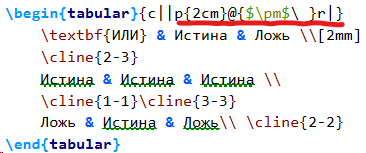
\includegraphics[width=0.7\linewidth]{screenshot001}
			\caption{}
			\label{fig:screenshot001}
		\end{figure}
		% TODO: \usepackage{graphicx} required
		\begin{figure}
			\centering
			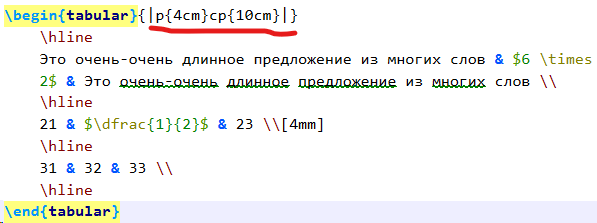
\includegraphics[width=0.7\linewidth]{screenshot002}
			\caption{}
			\label{fig:screenshot002}
		\end{figure}
		
	
\end{document} % Конец текста.